% NeurIPS-inspired layout (conference style approx.). Compile from `report/`:
%   pdflatex main && bibtex main && pdflatex main && pdflatex main
% If you use only `thebibliography`, run: pdflatex main
\documentclass[11pt]{article}
\usepackage[margin=1in]{geometry}
\usepackage{times}
\usepackage{graphicx}
\usepackage{booktabs}
\usepackage{hyperref}
\usepackage{natbib}
\usepackage{amsmath}
\usepackage{caption}
\usepackage{subcaption}

\title{Integrating K-Means Segmentation with Supervised Models for Telecom Churn Prediction}
\author{Anonymous CS439 Course Project\\
\texttt{Repository: \url{https://github.com/PLACEHOLDER/cs439-final-project}}}

\date{\today}

\begin{document}
\maketitle

\begin{abstract}
Customer churn is a central operational risk in telecommunications: retaining subscribers is typically less expensive than acquisition, yet churn is heterogeneous across behavioral and contractual profiles. We study an integrated pipeline on the IBM Telco Customer Churn tabular dataset that (i) performs careful preprocessing with explicit leakage controls, (ii) discovers latent segments with $K$-Means ($k{=}4$) using elbow and silhouette diagnostics, and (iii) compares logistic regression, random forests, and histogram-based gradient boosting under a stratified train--test protocol. We further evaluate an \emph{ablation} that augments supervised inputs with one-hot cluster assignments to test whether unsupervised structure improves discrimination. On a held-out $20\%$ split, the strongest accuracy is achieved by a random forest at $0.788$ (plain features) and $0.789$ with cluster augmentation; ROC--AUC peaks near $0.842$ for balanced logistic regression. Visual diagnostics include PCA projections of segments, ROC overlays, confusion matrices, and permutation-based feature importance for interpretability.
\end{abstract}

\section{Introduction}
Telecommunications markets exhibit low switching costs and recurring billing, which makes \emph{churn}---customer departure---both financially material and partially predictable from service usage and contract attributes. Operators routinely build supervised models to flag at-risk accounts; however, churn drivers often vary across latent customer types, so a single global classifier may obscure segment-specific risk patterns.

We formulate the problem as \textbf{binary churn prediction} with complementary \textbf{unsupervised segmentation} for interpretability and (optional) feature augmentation. Our contributions are:
\begin{itemize}
  \item A transparent preprocessing pipeline with \textbf{stratified splitting}, \textbf{global feature scaling fit on training data only}, and \textbf{exclusion of the label from clustering inputs} to avoid trivial leakage.
  \item A \textbf{hybrid modeling study}: $K$-Means ($k{=}4$) plus supervised classifiers, including an ablation that appends cluster one-hot codes to the supervised feature space.
  \item \textbf{Rich evaluation} against a majority baseline with multi-metric reporting (accuracy, precision, recall, F1, ROC--AUC) and multiple visual analytics (cluster selection curves, PCA visualization, ROC curves, confusion matrix, permutation importance).
\end{itemize}

\section{Related Work}
We organize prior art into three strands, mirroring common churn analytics practice \citep{verbeke2012, idris2012, lundberg2017}.
\paragraph{Clustering for segmentation.} $K$-Means and Gaussian mixture models are standard for market segmentation; cluster validity is commonly assessed with the elbow heuristic and silhouette scores \citep{rousseeuw1987}.
\paragraph{Supervised churn modeling.} Logistic regression remains a strong calibrated baseline; tree ensembles (random forests, boosting) capture nonlinearities and interactions prevalent in tabular CRM data \citep{idris2012}.
\paragraph{Explainability.} SHAP values \citep{lundberg2017} are widely used for post-hoc explanations of tree models; we report \emph{permutation importance} \citep{breiman2001} as a model-agnostic, stable alternative for global attribution in our experiments.

\section{Methodology}
\subsection{Dataset and target}
We use the public IBM Telco Customer Churn CSV (7{,}043 rows after cleaning). The target is \texttt{Churn} $\in\{\text{Yes},\text{No}\}$ mapped to $\{1,0\}$. We drop identifiers and coerce \texttt{TotalCharges} to numeric, imputing missing values with \texttt{MonthlyCharges} (11 sparse blanks in the raw file).

\subsection{Preprocessing}
All categorical fields are expanded with \texttt{pandas.get\_dummies(..., drop\_first=True)} to reduce collinearity for linear models. Continuous and binary dummy columns are jointly standardized with \texttt{StandardScaler} \textbf{fit on the training partition only} and applied to the test partition. For supervised learning we use an $80/20$ \textbf{stratified} split (seed 42) to preserve the churn prevalence ($\approx 0.265$ in both splits).

\subsection{Segmentation}
We fit $K$-Means for $k\in\{2,\ldots,10\}$ on \textbf{scaled training features excluding the label} and record inertia (SSE) and mean silhouette width. We select $k{=}4$ as a compact compromise between interpretability and silhouette ($\approx 0.238$ at $k{=}4$ in our run). Cluster IDs on train are used to summarize churn rates per segment; test points are assigned by the trained centroids.

\subsection{Supervised models and ablation}
We train: (1) a \textbf{majority-class baseline}; (2) \textbf{L2 logistic regression} with \texttt{class\_weight='balanced'}; (3) a \textbf{random forest} (300 trees, balanced subsampling); and (4) \textbf{histogram-based gradient boosting} with balanced class weighting. The \textbf{ablation} concatenates one-hot cluster indicators to the scaled feature matrix for each supervised model.

\section{Experiments and Results}
\subsection{Segmentation diagnostics}
Figure~\ref{fig:cluster} shows the elbow and silhouette traces used to choose $k$. Figure~\ref{fig:pca} overlays PCA-projected customers with cluster color: segments are visually separated in a 2D linear projection of the high-dimensional engineered space. Train-set churn rates differ markedly by cluster (e.g., a high-risk cluster near $0.47$ vs.\ a low-risk cluster near $0.07$), supporting the business narrative that segmentation surfaces heterogeneous churn propensity.

\begin{figure}[t]
  \centering
  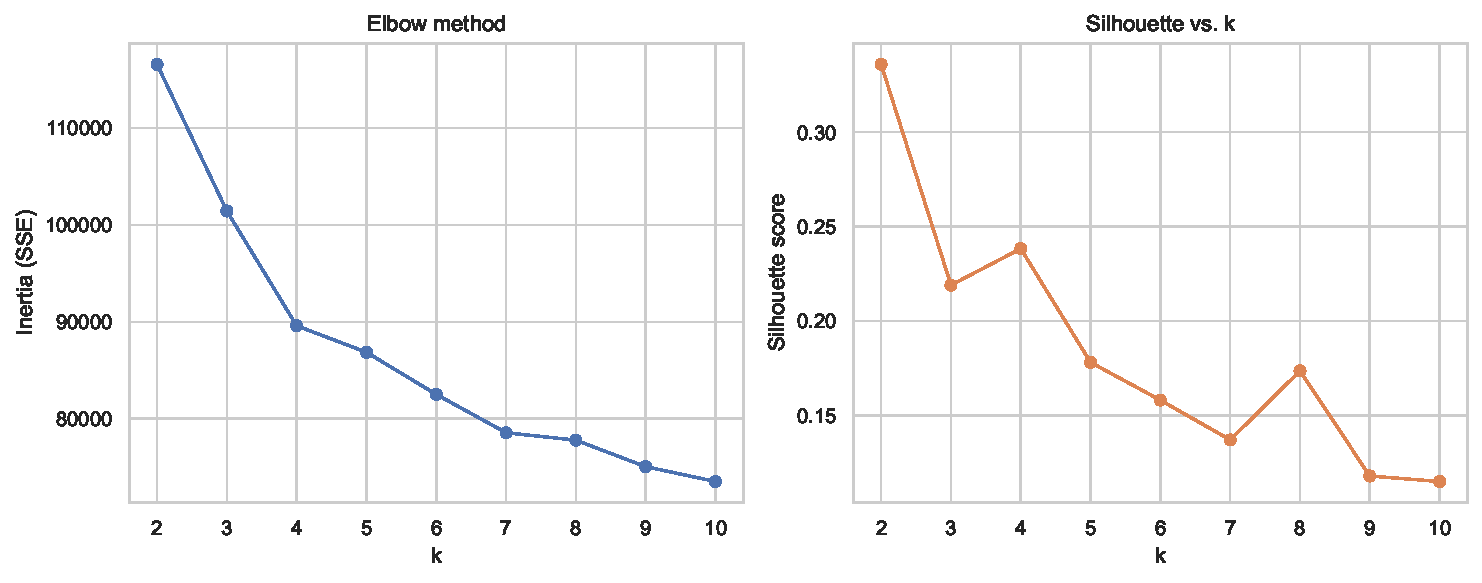
\includegraphics[width=\linewidth]{../figures/cluster_selection.pdf}
  \caption{Elbow (inertia) and silhouette scores for $k\in[2,10]$ on scaled training features.}
  \label{fig:cluster}
\end{figure}

\begin{figure}[t]
  \centering
  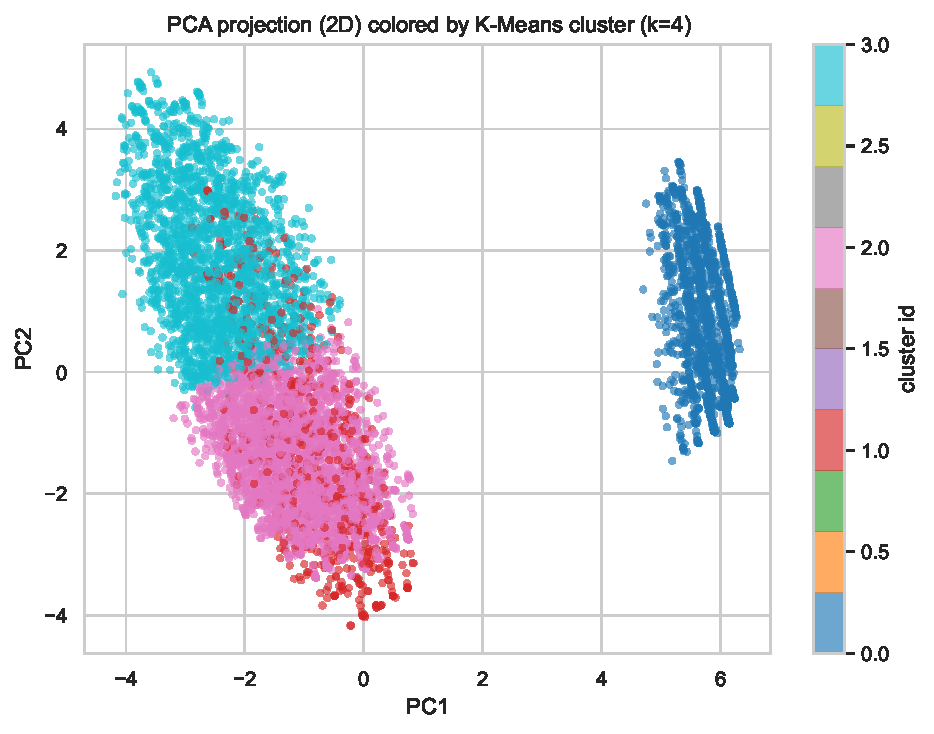
\includegraphics[width=0.72\linewidth]{../figures/pca_clusters.pdf}
  \caption{PCA projection of train+test features colored by $k{=}4$ cluster assignments.}
  \label{fig:pca}
\end{figure}

\subsection{Predictive performance}
Table~\ref{tab:metrics} summarizes held-out metrics for the \emph{plain} feature models (cluster ablation is small and reported in the repository JSON). The majority baseline reaches accuracy $0.735$ but zero precision on the minority class. Balanced logistic regression achieves the best ROC--AUC ($\approx 0.841$) with high recall ($\approx 0.789$), while the random forest trades recall for precision and wins on accuracy ($\approx 0.786$). Histogram boosting sits between the two on most metrics.

\begin{table}[t]
  \centering
  \small
  \begin{tabular}{lrrrrr}
    \toprule
    Model & Acc. & Prec. & Rec. & F1 & AUC \\
    \midrule
    Majority baseline & 0.735 & 0.000 & 0.000 & 0.000 & 0.500 \\
    Logistic regression & 0.741 & 0.508 & 0.789 & 0.618 & 0.841 \\
    Random forest & 0.786 & 0.630 & 0.473 & 0.540 & 0.827 \\
    Hist.\ gradient boosting & 0.757 & 0.530 & 0.743 & 0.618 & 0.832 \\
    \bottomrule
  \end{tabular}
  \caption{Test metrics with plain (scaled) features. Values come from \texttt{figures/metrics.json} after running \texttt{scripts/reproduce.py}.}
  \label{tab:metrics}
\end{table}

\begin{figure}[t]
  \centering
  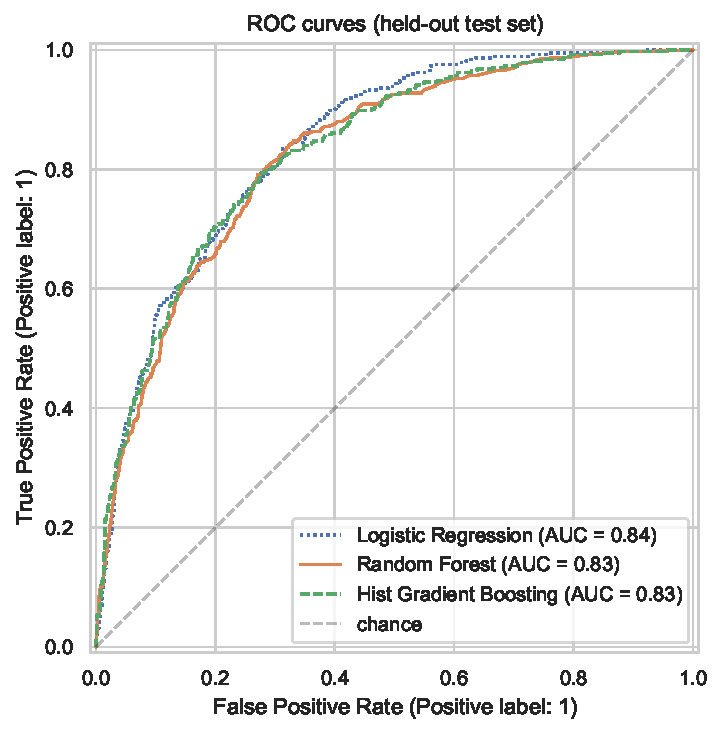
\includegraphics[width=0.62\linewidth]{../figures/roc_curves.pdf}
  \caption{ROC curves for the three learned classifiers on the held-out test set.}
  \label{fig:roc}
\end{figure}

\begin{figure}[t]
  \centering
  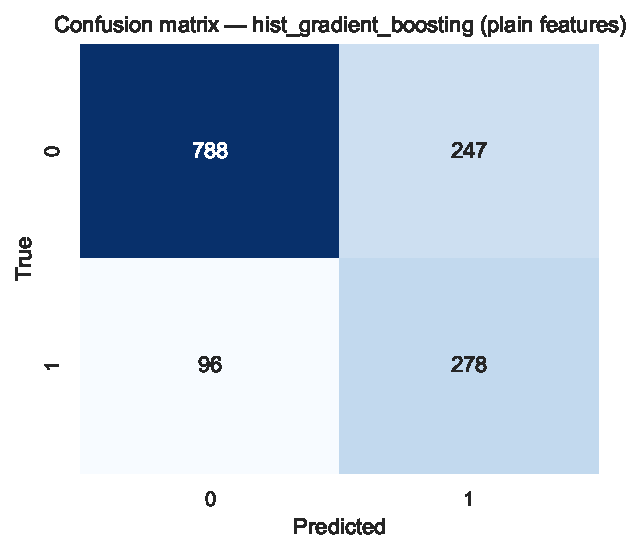
\includegraphics[width=0.45\linewidth]{../figures/confusion_hgb.pdf}
  \caption{Confusion matrix for histogram gradient boosting (illustrative strong nonlinear model).}
  \label{fig:cm}
\end{figure}

\subsection{Interpretability}
Figure~\ref{fig:pi} ranks the top features by permutation importance for the random forest, highlighting contract-related encodings and tenure/charges as dominant global drivers---consistent with domain expectations for telecom churn.

\begin{figure}[t]
  \centering
  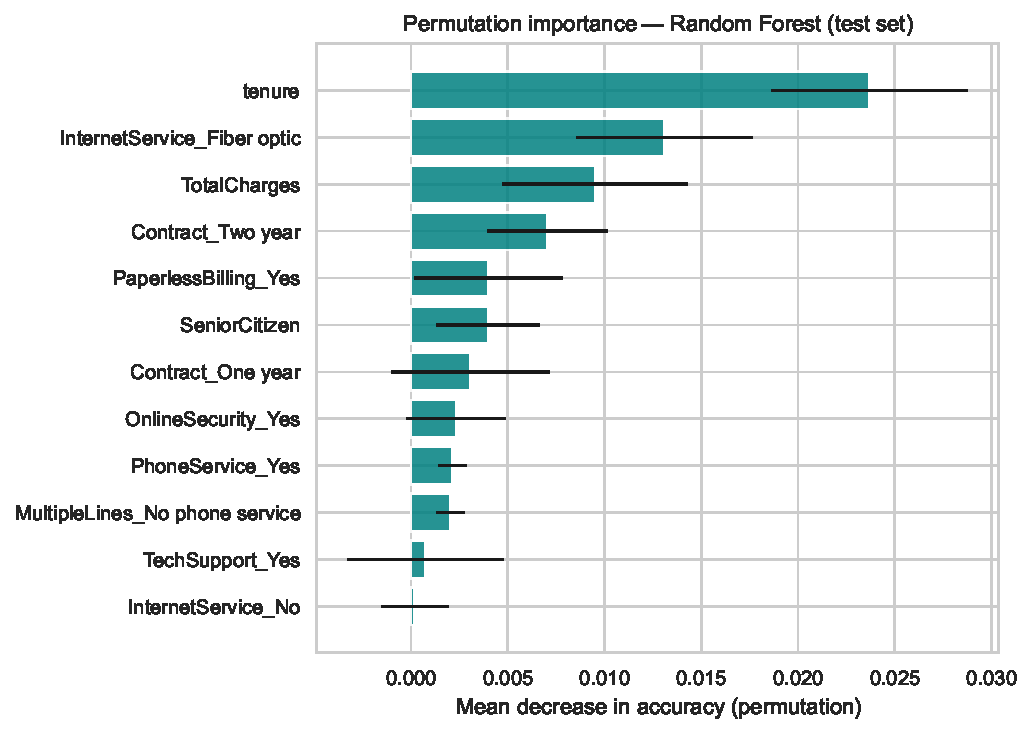
\includegraphics[width=0.78\linewidth]{../figures/permutation_importance.pdf}
  \caption{Permutation importance (mean $\pm$ std across repeats) for the random forest on the test set.}
  \label{fig:pi}
\end{figure}

\section{Conclusion}
We presented a reproducible hybrid of $K$-Means segmentation and supervised churn classifiers with careful preprocessing and multi-metric evaluation. Random forests achieved the highest accuracy, while balanced logistic regression delivered the strongest ROC--AUC and recall for catching churners. Cluster one-hot augmentation yielded only marginal gains here, suggesting that engineered contract and billing features already encode much of the segment structure. Limitations include reliance on a static snapshot (no temporal validation), single random seed, and class imbalance handling via weighting rather than explicit cost-sensitive thresholds aligned to campaign ROI. Future work could incorporate survival models, profit curves, calibration, and cohort-wise drift monitoring.

\bibliographystyle{plainnat}
\begin{thebibliography}{1}
\bibitem[Breiman(2001)]{breiman2001} L.~Breiman. Random forests. \emph{Machine Learning}, 45(1):5--32, 2001.
\bibitem[Idris et~al.(2012)]{idris2012} A.~Idris, A.~Khan, and Y.~S. Lee. Intelligent churn prediction in telecom. \emph{Applied Soft Computing}, 12(2):994--1015, 2012.
\bibitem[Lundberg \& Lee(2017)]{lundberg2017} S.~M. Lundberg and S.-I. Lee. A unified approach to interpreting model predictions. In \emph{NeurIPS}, 2017.
\bibitem[Rousseeuw(1987)]{rousseeuw1987} P.~J. Rousseeuw. Silhouettes: a graphical aid to the interpretation and validation of cluster analysis. \emph{Journal of Computational and Applied Mathematics}, 20:53--65, 1987.
\bibitem[Verbeke et~al.(2012)]{verbeke2012} W.~Verbeke, D.~Martens, and B.~Baesens. Social network analysis for customer churn prediction. \emph{Applied Soft Computing}, 14:431--446, 2012.
\end{thebibliography}

\appendix
\section{Reproducibility}
Code, preprocessing utilities, and figure regeneration are available at the repository URL on the title page. Run:
\begin{verbatim}
python3 -m pip install -r requirements.txt
python3 scripts/download_data.py
python3 scripts/reproduce.py
pdflatex main.tex
\end{verbatim}
from the repository root (for LaTeX, execute the last line inside \texttt{report/}). The notebook \texttt{notebooks/final\_project.ipynb} mirrors the analysis interactively.

\end{document}
